
\section{Data Types}
\markright{\arabic{section}. Data Types}
Like other Lisps, it is data objects that are typed, not variables.
Any variable can have any object as its value.
Although it is possible to
declare the type of object which is bound to a variable, but usually
it is only advisory information to the compiler to generate faster code.
Numbers are represented as immediate values in pointers and all the others
are represented by objects referenced by pointers.

In the implementation of Sun4, a pointer or a number is represented by
a long word as depicted in fig.\ref{Pointer}.
Two bits at LSB of a pointer are used as tag bits to discriminate
between a pointer, an integer, and a float.
Since a pointer's tags are all zero and it can use all 32 bits for
addressing an object, EusLisp can utilize up to 4GB of process
address space.

\begin{figure}[hb]
\begin{center}
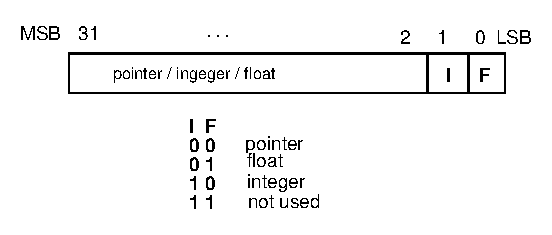
\includegraphics[width=10cm]{fig/pointer.ps}
% \epsfile{file=fig/pointer.ps}
%\mbox{
%\epsfxsize=10cm
%\epsfbox{fig/pointer.ps}
%}
\end{center}
\caption{\label{Pointer}Pointer and Immediate Value}
\end{figure}

\subsection{Numbers}

There are two kinds of numbers,
integer and float (floating-point number), both are represented
with 29 bits value and 1 bit sign.
Thus, integers range from -536,870,912 to 536,870,911.
Floats can represent plus/minus from 4.8E-38 to 3.8E38 with the
approximate accuracy of 6 digits in decimal, i.e.,
floating-point epsilon is approximately 1/1,000,000.

Numbers are always represented by immediate data, and not by objects.
This is the only exception of EusLisp's object orientation.
However, since numbers never waste heap memory, number crunching applications
run efficiently without causing garbage collection.

EusLisp does not have the character type,
and characters are represented by integers.
In order to write a program independent of character code sets,
%\#$\backslash$
\verb+#\+ reader dispatch macro is used.
However, when the character is read,
it is converted to numerical representation, and the printer does not
know how to reconvert it to
%\#$\backslash$
\verb+#\+ notation.

A number has two tag bits in a long word {Figure \ref{Pointer}},
which must be stripped off by shifting or masking 
when used in arithmetic computation.
Note that an integer should ignore two MSB bits by arithmetic shifting,
while a float should ignore two LSB bits by masking.
Byte swap is also necessary for an architecture like VAX which does not use
the rightmost byte as the least-significant mantissa byte.


\subsection{Objects}
Every data  other than number is represented by an object which is allocated
in heap. 
Each memory cell of an object has the object header and fixed number of 
slots for object variables.
Since vectors may consist of arbitrary number of elements,
they have 'size' slot immediately after the header.
Fig. \ref{ObjectFig} depicts the structures of object and vector, and their
header word.
Only the words indicated as {\em slot} and {\em element}
are accessible from users.

\begin{figure}[hbt]
\begin{center}
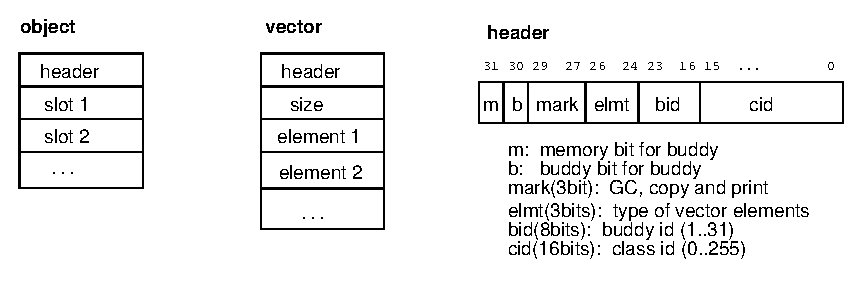
\includegraphics{fig/object.ps}
%\epsfile{file=fig/object.ps}
\end{center}
\caption{\label{ObjectFig}Structures of object, vector, and object header}
\end{figure}

A header is composed of six fields.
Two MSB bits, {\em m} and {\em b},
are used to indicate the side of the neighbor cell
in Fibonacci-buddy memory management.
There are three mark bits in the {\em mark} field, each of which
is used by the garbage collector to identify accessible cells,
by the printer to recognize circular objects in printing in {\tt \#n=} and
{\tt \#n\#} notations,
and by {\bf copy-object} to copy shared objects.
The {\em elmt} field discriminates one of seven possible data types
of vector elements, {\em pointer, bit, character, byte, integer, float}
and {\em foreign-string}.
Although {\em elmt} can be available in the class, 
it is provided in the header to make the memory manager independent of
the structure of a class and to make the element accessing faster.
The {\em bid} field represents the physical size of a memory cell.
31 different sizes up to 16 MB are represented by the five bits in this field.
%with relatively finer resolution than the binary buddy method.
The lower short word (16 bits) is used for the class id.
This is used to retrieve the class of an object via the system's class table.
This class id can be regarded as the type tag of traditional Lisps.
Currently only the lower 8 bits of the cid are used and the upper 8 bits
are ignored.
Therefore, the maximum number of classes is limited to 256, though
this limit can be raised up to 65536 by reconfiguring the EusLisp to allocate
more memory to the system's class table.

\subsection{Class Hierarchy}

The data structure of objects are defined by classes,
and their behaviors are defined by methods in the classes.
In EusLisp, a few dozens of classes have already been 
defined in tree structured
hierarchy as depicted in fig. \ref{ClassHierarchy}.
You can browse the real inheritance structure by the 
{\bf class-hierarchy} function.
The class 'object' at the leftmost is the ultimate super-class of
all the classes in EusLisp.
User-defined classes can inherit any of these built-in classes.

\begin{figure}
\small
\begin{verbatim}
object
     cons
          queue
     propertied-object
          symbol   -----  foreign-pod
          package
          stream
               file-stream
               broadcast-stream
          io-stream ---- socket-stream
          metaclass
               vectorclass
                    cstructclass
          read-table
          array
          thread
          barrier-synch
          synch-memory-port
          coordinates
               cascaded-coords
                    body
                    sphere
                    viewing
                         projection
                              viewing2d
                              parallel-viewing
                              perspective-viewing
                    coordinates-axes
               viewport
          line --- edge --- winged-edge
          plane
               polygon
                    face
                    hole
               semi-space
          viewer
          viewsurface  ----- tektro-viewsurface
     compiled-code
          foreign-code
          closure
          load-module
     label-reference
     vector
          float-vector
          integer-vector
          string
               socket-address
               cstruct
          bit-vector
          foreign-string
     socket-port
     pathname
     hash-table
     surrounding-box
     stereo-viewing
\end{verbatim}
\normalsize
\caption{\label{ClassHierarchy}Hierarchy of Predefined Classes}
\end{figure}

A class is defined the {\bf defclass} macro or by the {\bf defstruct} macro.

\ptext{
(defclass class-name \&key \= :super \hspace{15mm} \= class \\
 \> :slots \> () \\
 \> :metaclass \> metaclass \\
 \> :element-type \> t \\
 \> :size  -1\\ ) \\
(defstruct struct-name slots...) \\
(defstruct (struct-name [struct-options ...]) \\
\hspace{25mm}        (slot-name1 [slot-option...]) \\
\hspace{25mm}        (slot-name2 [slot-option...]) \\
\hspace{25mm}         ...) \\}

Methods are defined by the {\bf defmethod} special form.
{\bf Defmethod} can appear any times for a particular class.

\ptext{
(defmethod class-name  \\
 (:method-name1 (parameter...) . body1) \\
 (:method-name2 (parameter...) . body2) \\
 ...)
}

Field definitions for most of built-in classes are found in
{\tt *eusdir*/c/eus.h} header file.
{\tt (describe)} {\em class}) gives the description
of all the slots in {\em class}, namely, super class, slot names,
slot types, method list, and so on.
Definitions of built-in classes follow.
Note that the superclass of class {\bf object} is NIL
since it has no super class.

\ptext{
(defclass {\bf object} :super {\bf NIL} :slots ())
}

\ptext{
(defclass {\bf cons} :super {\bf object} :slots (car cdr))
}

\ptext{
(defclass {\bf propertied-object} :super {\bf object} \\
 \hspace{20mm} \=   :slots (plist)) \hspace{10mm} ;property list \\
}

\ptext{
(defclass {\bf symbol} :super {\bf propertied-object} \\
\hspace{20mm} :slots (\=value \hspace{15mm} \= ;specially bound value \\
 \>      vtype \>                ;const(0),var(1),special(2)  \\
 \>      function \>             ;global func def \\
 \>      pname               \>  ;print name string \\
 \>      homepkg)) \>            ;home package \\}

\ptext{
(defclass {\bf foreign-pod} :super {\bf symbol} \\
\hspace{20mm} :slots (\=podcode \hspace{15mm} \= ;entry code \\
 \>      paramtypes \>      ;type of arguments  \\
 \>      resulttype)) \\}


\ptext{
(defclass {\bf package} :super {\bf propertied-object} \\
\hspace{20mm} :slots (\= names \hspace{15mm} \= ;list of package name and nicknames\\
\>                   uses \>  ;spread use-package list \\
\>                   symvector \> ;hashed obvector \\
\>                   symcount \>  ;number of interned symbols \\
\>                   intsymvector \> ;hashed obvector of internal symbols \\
\>                   intsymcount \>  ;number of interned internal symbols \\
\>                   shadows \> ;shadowed symbols \\
\>                   used-by)) \>  ;packages using this package \\}

\ptext{
(defclass {\bf stream} :super {\bf propertied-object} \hspace{20mm} \\
\hspace{20mm} :slots (\= direction \hspace{3mm} \= ;:input or :output, nil if closed \\
  \>                   buffer  \>  ;buffer string \\
  \>                   count \> ;current character index \\
  \>                   tail)) \>  ;last character index \\
}

\ptext{
(defclass {\bf file-stream} :super {\bf stream} \\
\hspace{20mm} :slots (\= fd \hspace{10mm} \= ;file descriptor (integer)\\
 \>                    fname))\> ;file name str; qid for msgq \\
}

\ptext{
(defclass {\bf broadcast-stream} :super {\bf stream}\\
\hspace{20mm} :slots (destinations)) \hspace{10mm} ;streams to which output is delivered}

\ptext{
(defclass {\bf io-stream} \= :super {\bf propertied-object}\\
\>        :slots (instream outstream))}

\ptext{
(defclass {\bf socket-stream} \= :super {\bf io-stream}\\
\>        :slots (address)) \hspace{20mm} ; socket address}

\ptext{
(defclass {\bf read-table}  :super {\bf propertied-object} \\
\hspace{20mm}      :slots (\= syntax \hspace{10mm} \= ; byte vector representing character types \\
\>\> ; 0:illegal, 1:white, 2:comment, 3:macro\\
\>\> ; 4:constituent, 5:single\_escape\\
\>\> ; 6:multi\_escape, 7:term\_macro, 8:nonterm\_macro \\
\> macro \> ;character macro expansion function\\
\> dispatch-macro)) \\}

\ptext{
(defclass {\bf array} :super {\bf propertied-object} \\
\hspace{20mm} :slots (\= entity \hspace{12mm}\= ;simple vector storing array entity \\
 \>           rank  \> ;number of dimensions: 0-7 \\
 \>           fillpointer \>    ;pointer to push next element \\
 \>           offset      \>    ;offset for displaced array \\
 \>           dim0,dim1,dim2,dim3,dim4,dim5,dim6))  ;dimensions \\}

\ptext{
(defclass {\bf metaclass} :super {\bf propertied-object} \\
\hspace{20mm}   :slots   (\= name  \hspace{8mm} \= ;class name symbol \\
 \>           super   \>   ;super class \\
 \>           cix  \>      ;class id \\
 \>           vars  \>     ;var name vector including inherited vars \\
 \>           types  \>    ;type vector of object variables \\
 \>           forwards \>  ;components to which messages are forwarded \\
 \>           methods))  \>  ;method list \\ }

\ptext{
(defclass {\bf vectorclass} :super {\bf metaclass}  \\
\hspace{20mm} :slots (\= element-type  \hspace{4mm} \= ;vector element type 0-7\\
 \>                 size)) \>  ;vector size; 0 if unspecified \\ }

\ptext{
(defclass {\bf cstructclass} :super {\bf vectorclass}  \\
\hspace{20mm} :slots (\= slotlist))  \hspace{4mm} \= ;cstruct slot descriptors\\
}

\ptext{
(defclass {\bf vector} :super {\bf object} :slots (size))}

\ptext{
(defclass {\bf float-vector} :super {\bf vector} :element-type :float)}

\ptext{
(defclass {\bf string} :super {\bf vector} :element-type :char)}

\ptext{
(defclass {\bf hash-table} :super {\bf propertied-object} \\
\hspace{20mm}  :slots   (\= lisp::key \hspace{20mm}\= ;hashed key vector\\
\> value \> ; value vector\\
\> size \> ; the size of the hash table\\
\> count \> ; number of elements entered in the table\\
\> lisp::hash-function \> \\
\> lisp::test-function \\
\> lisp::rehash-size \\
\> lisp::empty  lisp::deleted \>) \\
}

\ptext{
(defclass {\bf queue} :super {\bf cons})}

\ptext{
(defclass {\bf pathname} :super {\bf propertied-object} \\
\hspace{20mm}  :slots   (\= lisp::host device \hspace{20mm}\= ; not used\\
\> directory \> ; list of directories\\
\> name \> ; file name before the last "."\\
\> type \> ; type field after the last "."\\
\> lisp::version) \> ; not used \\
}

\ptext{
(defclass {\bf label-reference} \hspace{8mm}  ;for reading \#n=, \#n\# objects \\
\hspace{20mm} \= :super {\bf object} \\
\>   :slots (label value unsolved next)) \\}

\ptext{
(defclass {\bf compiled-code} :super {\bf object} \\
\hspace{20mm}  :slots   (\= codevector \\
 \>          quotevector \\
 \>          type \hspace{15mm} \=    ;0=func, 1=macro, 2=special \\
 \>          entry))  \>  ;entry offset }

\ptext{
(defclass {\bf closure} \= :super {\bf compiled-code} \\
\>              :slots (env1 env2));environment}

\ptext{
(defclass {\bf foreign-code}  :super {\bf compiled-code}  \\
\hspace{20mm}  :slots   (\= paramtypes  \hspace{10mm} \=  ;list of parameter types\\
 \>              resulttype)) \> ;function result type}

\ptext{
(defclass {\bf load-module}  :super {\bf compiled-code}  \\
 \hspace{15mm}  :slots  (\= symbol-table \hspace{3mm} \= ;hashtable of symbols defined \\
 \>         object-file \> ;name of the object file loaded, needed for unloading \\
 \>         handle \> ;file handle returned by ''dlopen''}

\subsection{Type Specifier}
Though EusLisp does not have the {\bfx deftype} special form,
type names are used in declarations and functions requesting
to specify the type of results or contents,
as in {\bf coerce, map, concatenate, make-array}, etc.
Usually, class names can be used as type specifiers, as in
{\tt (concatenate cons "ab" "cd") = (97 98 99 100)},
where Common Lisp uses {\tt (quote list)} instead of {\tt cons}.

As EusLisp does not have classes to represent numbers,
types for numbers need to be given by keywords.
{\bfx :integer}, {\bfx integer}, {\bfx :int}, {\bfx fixnum},
or {\bfx :fixnum} is used to represent the integer type,
{\bfx :float} or {\bfx float}, the floating point number type.
As the {\emx element-type} argument of {\bfx make-array},
{\bfx :character}, {\bfx character}, {\bfx :byte}, and {\bfx byte}
are recognized to make strings.
Low level functions such as {\bfx defcstruct}, {\bfx sys:peek},
and {\bfx sys:poke}, also recognize
{\bfx :character}, {\bfx character}, {\bfx :byte}, or {\bfx byte}
for the byte access, and {\bfx :short} or {\bfx short} for short word access.
In any cases, keywords are preferable to lisp package symbols with the
same pname.

\newpage

\section{Forms and Evaluation}
\markright{\arabic{section}. Forms and Evaluation}
\subsection{Atoms}

A data object other than a cons is always an atom, no matter what complex
structure it may have.
Note that NIL, which is sometimes noted as () to represent an empty
list, is also an atom.
Every atom except a symbol is always evaluated to itself,
although quoting is required in some other Common Lisp implementations.

\subsection{Scoping}

Every symbol may have associated value.
A symbol is evaluated to its value determined in the current binding context.
There are two kinds of variable bindings;
the lexical or static binding and the special or dynamic binding.
Lexically bound variables are introduced by {\bf lambda} form or
{\bf let} and {\bf let*} special forms
unless they are declared special.
Lexical binding can be nested and the only one binding which is introduced
innermost level is visible, hiding outer lexical bindings and the special 
binding.
Special variables are used in two ways:
one is for global variables, and the other is for dynamically scoped
local variables which are visible even at the outside of
the lexical scope as long as the binding is in effect.
In the latter case, special variables are needed to be declared special.
The declaration is recognized not only by the compiler, but also by
the interpreter.
According to the Common Lisp's terms, special variables are said to have
indefinite scope and dynamic extent.
%\footnote{In Maclisp, all the variables are taken to be special by the
%interpreter, and lexical by the compiler if not declared special.
%In Etalisp, all variables are special and no declaration is recognized.}

Even if there exists a lexical variable in a certain scope,
the same variable name can be redeclared to be special in inner scope.
Function {\bf symbol-value} can be used to retrieve  the special values
regardless to the lexical scopes.
Note that {\bf set} function works only for special variable, i.e.
it cannot be used to change the value of lambda or let variables
unless they are declared special.

\begin{verbatim}
(let ((x 1))
   (declare (special x))
   (let* ((x (+ x x)) (y x))
      (let* ((y (+ y y)) (z (+ x x)))
         (declare (special x))
         (format t "x=~S y=~s z=~s~%" x y z) ) ) )
--> x=1 y=4 z=2
\end{verbatim}

A symbol can be declared to be a constant by {\bf defconstant} macro.
Once declared, an attempt to change the value signals an error thereafter.
Moreover, such a constant symbol is inhibited to be used as
the name of a variable even for a local variable.
NIL and T are examples of such constants.
Symbols in the keyword package are always declared to be constants
when they are created.
In contrast, {\bf defvar} and {\bf defparameter} macro declare
symbols to be special variables.
{\bf defvar} initializes the value only if the symbol is unbound,
and does nothing when it already has a value assigned,
while {\bf defparameter} always resets the value.

When a symbol is referenced and there is no lexical binding for the symbol,
its special value is retrieved.
However, if no value has been assigned to its special value yet,
unbound variable error is signaled.

\subsection{Generalized Variables}
Generally, any values or attributes are represented in slots of objects
(or in stack frames).
To retrieve and alter the value of a slot,
two primitive operations, {\em access} and {\em update}, must be provided.
Instead of defining two distinct primitives for every slot of objects,
EusLisp, like Common Lisp, provides uniform update operations
based on the generalized variable concept.
In this concept, a common form is recognized  either as a value access form
or as a slot location specifier.
Thus, you only need to remember accessing form for each slot and
update is achieved by {\bf setf} macro used in conjunction with the access form.
For example, {\tt (car x)} can be used to replace the value
in the car slot of {\tt x} when used with {\bf setf} as in {\tt (setf (car 
'(a b) 'c)},
as well as to take the car value out of the list.

This method is also applicable to all the user defined objects.
When a class or a structure is defined, the access and update forms
for each slot are automatically defined.
Each of those forms is defined as a macro whose name is the concatenation of
the class name and slot name.
For example, car of a cons can be addressed by {\tt (cons-car '(a b c))}.

\begin{verbatim}
(defclass person :super object :slots (name age))
(defclass programmer :super person :slots (language machine))
(setq x (instantiate programmer))
(setf (programmer-name x) "MATSUI"
      (person-age x) 30)
(incf (programmer-age x))
(programmer-age x)   --> 31
(setf (programmer-language x) 'EUSLISP
      (programmer-machine x) 'SUN4)
\end{verbatim}

Array elements can be accessed in the same manner.

\begin{verbatim}
(setq a (make-array '(3 3) :element-type :float))
(setf (aref a 0 0) 1.0 (aref a 1 1) 1.0 (aref a 2 2) 1.0)
a --> #2f((1.0 0.0 0.0) (0.0 1.0 0.0) (0.0 0.0 1.0))

(setq b (instantiate bit-vector 10))  --> #*0000000000
(setf (bit b 5) 1)
b --> #*0000010000
\end{verbatim}

In order to define special setf methods for particular objects,
{\bf defsetf} macro is provided.

\begin{verbatim}
(defsetf symbol-value set)
(defsetf get (sym prop) (val) `(putprop ,sym ,val ,prop))
\end{verbatim}

\subsection{Special Forms}

\begin{table}
\begin{center}
{\large
\begin{tabular}{|l l l|} \hline 
and & flet & quote \\
block & function & return-from\\
catch & go & setq \\
cond & if & tagbody \\
declare & labels & the \\
defmacro & let & throw \\
defmethod & let* & unwind-protect \\
defun & progn & while \\
eval-when & or & \\
\hline
\end{tabular} }
\end{center}
\caption{\label{SpecialForms}EusLisp's special forms}
\end{table}

All the special forms are listed in Table \ref{SpecialForms}.
{\bf macrolet, compiler-let,} and {\bf progv} have not been implemented.
Special forms are essential language constructs for the management of
evaluation contexts and control flows.
The interpreter and compiler have special knowledge to
process each of these constructs properly, while the application
method is uniform for all functions.
Users cannot add their own special form definition.

\subsection{Macros}

Macro is a convenient method to expand language constructs.
When a macro is called, arguments are passed to the macro body,
which is a macro expansion function, without being evaluated.
Then, the macro expansion function expands the arguments,
and returns the new form.
The resulted form is then evaluated again outside the macro.
It is an error to apply a macro or special form to a list of arguments.
{\bf Macroexpand} function can be used for the explicit macro expansion.

Though macro runs slowly when interpreted,
it speeds up compiled code execution,
because macro expansion is taken at compile-time only once
and no overhead is left to run-time.
Note that explicit call to eval or apply in the macro function may
produce different results between interpreted execution
and the compiled execution.

\subsection{Functions}

A function is expressed by a lambda form which is merely a list
whose first element is {\bf lambda}.
If a lambda form is defined for a symbol using {\bf defun}, it can be referred
as a global function name.
Lambda form takes following syntax.

\ptext{
(lambda (\= \{var\}* \\
\>  [\&optional \{var $|$ (var [initform])\}*] \\
\>  [\&rest form] \\
\>  [\&key \= \{var $|$ (var [initform]) $|$ ((keyword var) [initform])\}* \\
\> \> [\&allow-other-keys]] \\
\>  [\&aux \{var $|$ (var [initform])\}*]) \\
 \hspace{10mm} \{declaration\}* \\
 \hspace{10mm} \{form\}*) \\
}

There is no function type such as EXPR, LEXPR, FEXPR, etc.:
arguments to a function are always evaluated before its application,
and the number of acceptable arguments is determined by lambda-list.
Lambda-list specifies the sequence of parameters to the lambda form.
Each of {\bf \&optional, \&rest, \&key } and {\bf \&aux} has special
meaning in lambda-lists, and these symbols cannot be used as variable
names.
Supplied-p variables for \&optional or \&key parameters are not supported.

Since a lambda form is indistinguishable from normal list data,
{\bf function} special form must be used to inform the interpreter and
compiler the form is intended to be a function.
\footnote{In CLtL-2 a quoted lambda form is no longer a function.
Application of such a form is an error.}
{\bf Function} is also important to freeze the environment onto the function,
so that all the lexical variables can be accessible in the function
even the function is passed to another function of different lexical scope.
The following program does not work either interpretedly nor after compiled,
since {\tt sum} from the {\tt let} is invisible  inside lambda form.

\begin{verbatim}
(let ((x '(1 2 3)) (sum 0))
  (mapc '(lambda (x) (setq sum (+ sum x))) x))
\end{verbatim}

To get the expected result, it should be written as follows:
\begin{verbatim}
(let ((x '(1 2 3)) (sum 0))
   (mapc #'(lambda (x) (setq sum (+ sum x))) x ))
\end{verbatim}

\#' is the abbreviated notation of {\bf function},
i.e. {\tt \#'(lambda (x) x)} is equivalent to
{\tt (function (lambda (x) x))}.
Here is another example of what is called a funarg problem:

\begin{verbatim}
(defun mapvector (f v)
    (do ((i 0 (1+ i)))
       ((>= i (length v)))
       (funcall f (aref v i))))
(defun vector-sum (v)
    (let ((i 0))
       (mapvector #'(lambda (x) (setq i (+ i x))) v)
       i))
(vector-sum #(1 2 3 4)) --> 10 
\end{verbatim}

EusLisp's closure cannot have indefinite extent:
i.e. a closure can only survive as long as its outer extent is in effect.
This means that a closure cannot be used for programming of ``generators".
The following program does not work.

\begin{verbatim}
(proclaim '(special gen))
(let ((index 0))
   (setq gen #'(lambda () (setq index (1+ index)))))
(funcall gen)
\end{verbatim}

However, the same purpose is accomplished by object oriented programming,
because an object can hold its own static variables:
\begin{verbatim}
(defclass generator object (index))
(defmethod generator
 (:next () (setq index (1+ index)))
 (:init (&optional (start 0)) (setq index start) self))
(defvar gen (instance generator :init 0))
(send gen :next)
\end{verbatim}
\newpage
